\documentclass{article}
\usepackage[utf8]{inputenc}
\usepackage{graphicx}
\usepackage{caption}
\usepackage{subcaption}
\usepackage{float}
\usepackage{listings}
\usepackage[margin=1in]{geometry}
\title{Project 01: Networking}
\author{J. Patrick Lacher {\textless}jlacher1@nd.edu{\textgreater}
\\Nicholas Carroll {\textless}ncarroll@nd.edu{\textgreater}
\\James Marvin {\textless}jmarvin1@nd.edu{\textgreater}}


\begin{document}

\maketitle


\section{Summary}

\paragraph{}

In this project, we created two python scripts to learn about networking in the creation of python, as well as the better understand the ideas of child and Parent processes.  Our first script, \textbf{thor.py}, named for its ability to  "hammer" the web was designed to act in a similar manner to a curl or wget function, as it would retrieve the data stored at a particular address and measure the time to took to retrieve said data. Our second script, called \textbf{spidey.py}, was designed to dynamically "spin up" websites, listen on ports and then have then accessible and be able to process requests to display directories, run scripts, and handle errors.  These two tasked would then be used in conjunction with one another to measure the latency and the throughput of our server both in forking and non-forking mode.  These tasks was worked out by assigning different members particular functions or tasks (i.e. request parsing, argument processing, forking, etc) and then combining the different elements to make sure they worked together.  Things that didn't work particularly well for us in the project included test scripts.  We thought we finished the project completely, but making the test scripts proved particularly problematic this was not only because writing the test scripts proved particularly troublesome, but they revealed problems with our code that we didn't fully realize until we ran the test scripts.  


\section{Latency}

\paragraph{}

Latency is essentially the speed of a request on-line. It can be measured with a ping command from a UNIX machine, but for the sake of our experiment we are going to use the \textbf{thor.py} script that we ran.  to test latency, we ran \textbf{thor.py} on the script page, the directory listing pages, and static files while the server was in both forking and non-forking mode.  We then averaged the data together so we could analyze it.  

\begin{figure}[H]
    \centering
    \begin{subfigure}{.5\textwidth}
        \centering
        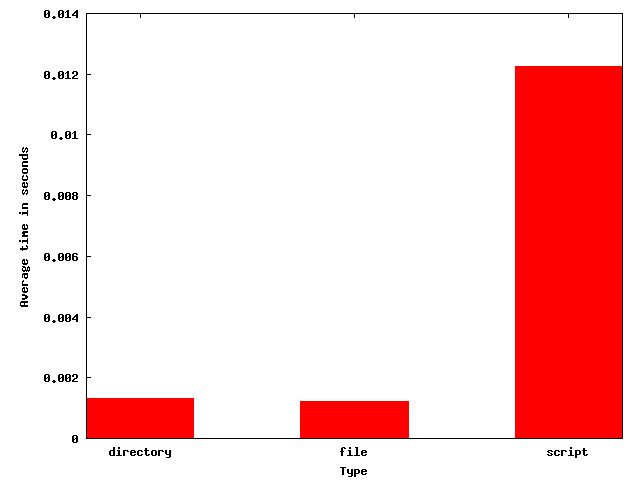
\includegraphics[scale=0.18]{latency.png}
        \caption{Without Forking (Single-Response)}
        \label{fig:1.1}
    \end{subfigure}%
    \begin{subfigure}{.5\textwidth}
         \centering
        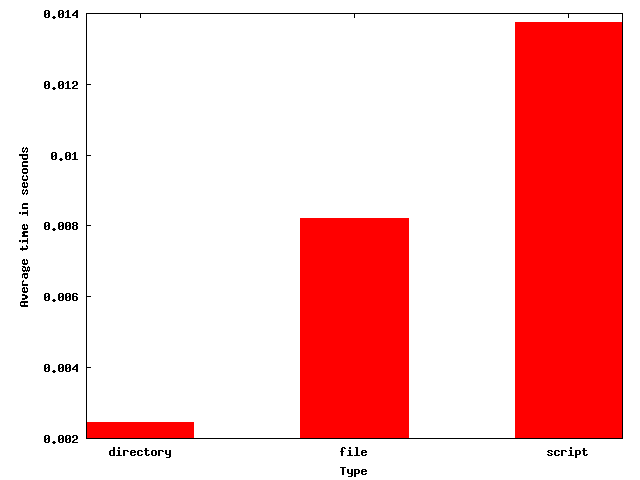
\includegraphics[scale=0.18]{latencywithfork.png}
        \caption{With Forking (Multi-Response)}
        \label{fig:1.2}
    \end{subfigure}%
    \caption{Server Latency}
    \label{fig:1}
\end{figure}

\section{Throughput}

\paragraph{}

Throughput is essentially the amount of content that can flow in/out in a particular moment of time, much like the volume of water that can pass through a pipe at a particular moment.  To measure this on the computer, you normally test the amount of time it takes to retrieve a file of a particular size.  to test this out we created three dummy files of various sizes and then compared the average speed to retrieve them with \textbf{thor.py} in both forking and non-forking mode.  we then compiled the data so we could analyze it. 

\begin{figure}[H]
    \centering
    \begin{subfigure}{.5\textwidth}
        \centering
        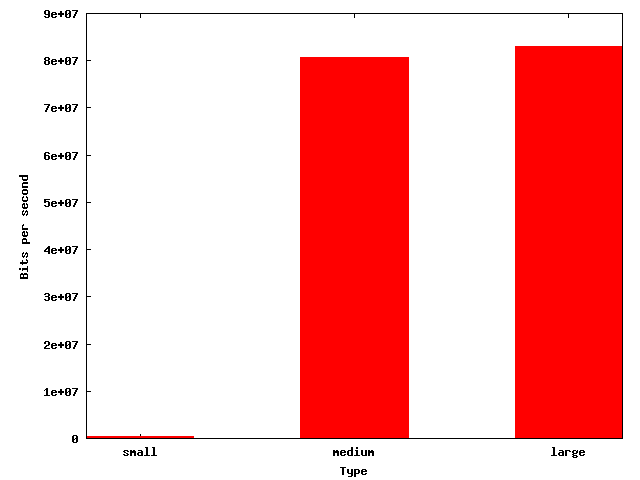
\includegraphics[scale=0.18]{throughput.png}
        \caption{Without Forking (Single-Response)}
        \label{fig:1.1}
    \end{subfigure}%
    \begin{subfigure}{.5\textwidth}
         \centering
        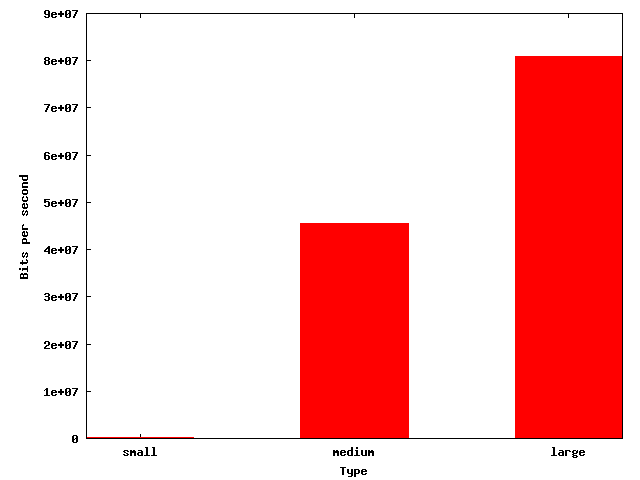
\includegraphics[scale=0.18]{throughputwithfork.png}
        \caption{With Forking (Multi-Response)}
        \label{fig:1.2}
    \end{subfigure}%
    \caption{Server Throughput (bytes/sec)}
    \label{fig:1}
\end{figure}

\section{Analysis}

\paragraph{}

The first experiment called for testing latency on \textbf{spidey.py} using \textbf{thor.py} to measure latency for files, directories, and scripts in both forking and non-forking mode. The results, available above in \textbf{Figure 1}, show that the server latency is much higher for scripts than for either of the other options due to the extra processing required to render information from scripts. The results also showed that the non-forking configuration of the server has much lower latency, a result of diverting all processing resources to filling a single request. A forking model adds the ability to simultaneously handle multiple requests, but suffers greater latency as a result of the divided resources.

\paragraph{}
The second experiment called for testing server throughput in a similar fashion to latency, the results of which can be seen in \textbf{Figure 2} above. Both methods (forking and non-forking) had very high throughputs for the large files, but there was a noticeable drop in throughput for the smaller files in forking mode, again a result of divided resources when the server is deployed to field multiple requests.

\section{Conclusion}

\paragraph{}
 
Overall we learned how to host and make requests to a server. These skills will hopefully prove useful when we have to create web based applications in the future. Thor and Spidey illustrated on a small scale what happens on the web billions of times a day. This assignment showed us another powerful feature of python programming. It also made us more aware of the power of friendship and group coding. 

\end{document}